\documentclass{beamer}
\usepackage[utf8]{inputenc}
\usepackage[english,russian]{babel}

\usepackage{xcolor}

\usepackage{amsmath,amsfonts,amssymb,amsthm,amscd,amsxtra}
\usepackage{physics}
\usepackage[sharp]{easylist}
\usepackage{comment}
\usepackage{mathtools} % xmapsto, \Vector

\usepackage[backend=biber,bibencoding=utf8,sorting=none,sortcites=true,bibstyle=sty/gost71,maxnames=99,citestyle=numeric-comp,babel=other]{biblatex
}
\addbibresource{thesis.bib}

\usepackage{beamerthemesplit}
\usetheme{Boadilla}
\setbeamertemplate{caption}[numbered]

% \usepackage[pdftex]{graphicx}
\graphicspath{ {pic/} }
\usepackage{tikz}

\newcommand{\hilb}[1]{\mathcal{H}_{#1}}
\newcommand{\cconj}[1]{\overline{#1}}
\newcommand{\hank}[1]{H_{#1}^{(1)}}

\newcommand{\mcF}{\mathcal{F}}
\newcommand{\mcH}{\mathcal{H}} % ???
\newcommand{\mcI}{\mathcal{I}}
\newcommand{\mcL}{\mathcal{L}} % L2 space
\newcommand{\mcO}{\mathcal{O}} % Big O
\newcommand{\mcP}{\mathcal{P}}


\newcommand{\bbC}{\mathbb{C}} % complex plane
\newcommand{\bbD}{\mathbb{D}} % complex unit disk
\newcommand{\bbH}{\mathbb{H}} % complex upper half-plane TODO add to template
\newcommand{\bbN}{\mathbb{N}}
\newcommand{\bbK}{\mathbb{K}}
\newcommand{\bbR}{\mathbb{R}}
\newcommand{\bbT}{\mathbb{T}} % complex unit circle
\newcommand{\bbZ}{\mathbb{Z}}

\newcommand{\eqdef}{\overset{\mathrm{def}}{=\joinrel=}}

\DeclareMathOperator{\dom}{dom}
\DeclareMathOperator{\ran}{Ran}
\DeclareMathOperator{\rng}{rng}

\newcommand{\todo}[1]{\textcolor{red}{{\large TODO: #1}}}

\newenvironment{elist}{\begin{easylist}[enumerate]}{\end{easylist}}
\newenvironment{ilist}{\begin{easylist}[itemize]}{\end{easylist}}

\newcommand{\myspecial}[1]{\mathrm{#1}}

% imaginary unit
\newcommand{\iu}{{i\mkern1mu}}


\newcommand{\ipcdot}{\ip{\cdot}{\cdot}}
\newcommand{\iip}[2]{[#1,#2]}
\newcommand{\iipcdot}{\iip{\cdot}{\cdot}}

\newcommand{\dsum}{\oplus}
\newcommand{\ddiff}{\ominus}
% indefinite direct sum
\newcommand{\idsum}{[+]}
\newcommand{\iddiff}{[-]}

\DeclarePairedDelimiter{\Vector}{\lparen}{\rparen}

\newcommand{\tit}{\textit}
\newcommand{\cls}{\overline}
\newcommand{\eps}{\varepsilon}


\newcommand{\argmin}{\operatornamewithlimits{argmin}}
\newcommand{\argmax}{\operatornamewithlimits{argmax}}

\renewcommand{\Re}{\operatorname{Re}}
\renewcommand{\Im}{\operatorname{Im}}
\renewcommand{\phi}{\varphi} % TODO is there a prettier way to do that

\newcommand{\eexp}[1]{e^{#1}}

\DeclareMathOperator\atanh{atanh}

% ???
% \newcommand{\abs}[1]{\left| #1 \right|}
% \newcommand{\norm}[1]{\left\lVert #1 \right\rVert}
\newcommand*\Eval[3]{\left.#1\right\rvert_{#2}^{#3}}

\title[]{Исследование полноты резонансных состояний оператора Шредингера
для модели квантовых графов}
\author[Дмитрий Герасимов]{Дмитрий Герасимов\\{\small научный руководитель: \\ д.ф.-м.н., профессор кафедры ВМ, И.Ю.Попов}}
\institute[ИТМО]{Университет ИТМО}
\date{11 июня 2016 года}

\begin{document}

\maketitle

\begin{frame}{Полнота резонансных состояний}

\begin{itemize}
\item Задача полноты важна как в теории, так и на практике.
% Задача полноты важна и с теоретической точки зрения (теория функций, дифференциальные уравнения), так и с практической (возможность разложить состояния в ряд Фурье, аппроксимации и т.п.)

\item Рассматриваем резонатор Гельмгольца и оператор Шредингера с граничным условием Дирихле или Неймана (чисто дискретный спектр).
% Рассматривается некий резонатор, оператор Шредингера с граничным условием Дирихле в нем имеет чисто дискретный спектр, набор собственный функций полон в $\mcL^2(\Omega)$.

\item Применяем возмущение, соединяя резонатор с волноводом (дискретный спектр смещается в резонансы)

\item Интересным вопросом является нахождение области, на котором резонансные состояния полны. \textbf{Гипотеза: на выпуклой оболочке рассеивателя}.
\end{itemize}
% 
% Далее, рассматриваем возмущение этой задачи, соединяя резонатор с волноводом через небольшое отверстие. После этого дискретный спектр пропадает, а собственные значения «смещаются» в комплексную плоскость и становятся резонансами. Резонансные состояния формально удовлетворяют уравнению Шредингера и граничным условиям, однако не принадлежат L^2(Gamma). С другой стороны, при ограничении их на конечный домен Omega, они лежат в L^2(Omega). 
\end{frame}



% SAY: сказать тут, как вообще выглядит модель, свободное уравнение Шредингера, рассеиватель и т.п.
\begin{frame}{Существующие результаты}
\begin{figure}
\begin{tikzpicture}[scale=0.8]
\newcommand{\Wglen}{10.0}; % waveguide length

\coordinate (LLL) at (-\Wglen - 1, 0);
\coordinate (RRR) at ( \Wglen + 1, 0);
\coordinate (LL)  at (-\Wglen, 0);
\coordinate (RR)  at ( \Wglen, 0);
% change these to take resonator length into account
\coordinate (L)   at (0, 0);
\coordinate (R)   at (0, 0);
%

\coordinate (U) at (0, 3); % upper point of resonator

% waveguide
\draw[ultra thick, dotted] (LLL) -- (LL);
\draw[ultra thick] (LL)--(L);
\draw[ultra thick] (R)--(RR);
\draw[ultra thick, dotted] (RR) -- (RRR);
%

\draw[<-] (-\Wglen + 1, 2) -- (-\Wglen + 5, 2) node [midway, above] {$R e^{-\iu k x}$};
\draw[->] (-\Wglen + 1, 0.5) -- (-\Wglen + 5, 0.5) node [midway, above] {$e^{\iu k x}$};
\draw[->] (\Wglen - 5, 0.5) -- (\Wglen - 1, 0.5) node [midway, above] {$T e^{\iu k x}$};

\draw[ultra thick] node [below] {$V$} (0, 0) -- node [left] {$\Omega$} (U);
\end{tikzpicture}
\caption{Одномерный резонатор-отрезок с $\delta$-условием в $V$}
\end{figure}
\end{frame}



\begin{frame}{Существующие результаты}
\begin{figure}
\begin{tikzpicture}[scale=0.8]
\newcommand{\Wglen}{6.0}; % waveguide length
\newcommand{\Warrlen}{2.0}; % wave arrow length
\newcommand{\Reslen}{2.0}; % resonator length

\coordinate (LLL) at (-\Wglen - 1, 0);
\coordinate (RRR) at ( \Wglen + 1, 0);
\coordinate (LL)  at (-\Wglen, 0);
\coordinate (RR)  at ( \Wglen, 0);
\coordinate (L)   at (-\Reslen, 0);
\coordinate (R)   at ( \Reslen, 0);
%

\coordinate (U) at (0, 3); % upper point of resonator

% waveguide
\draw[ultra thick, dotted] (LLL) -- (LL);
\draw[ultra thick] (LL)--(L);
\draw[ultra thick] (R)--(RR);
\draw[ultra thick, dotted] (RR) -- (RRR);
%

\draw[<-, thick] (-\Wglen, 1.5) -- (-\Wglen + \Warrlen, 1.5) node [midway, above] {\large $R e^{-\iu k x}$};
\draw[->, thick] (-\Wglen, 0.8) -- (-\Wglen + \Warrlen, 0.8) node [midway, above] {\large $e^{\iu k x}$};
\draw[->, thick] (\Wglen - \Warrlen, 0.5) -- (\Wglen, 0.5)   node [midway, above] {\large $T e^{\iu k x}$};

\draw (LL) node [below] {\large $\Omega_L$};
\draw (RR) node [below] {\large $\Omega_R$};

\draw[ultra thick] (0, 2) node [above] {\Large $\Omega$};

\draw (-2,0) arc (180:360:2cm and 0.5cm);
\draw[dashed] (-2,0) arc (180:0:2cm and 0.5cm);
\draw (0,2) arc (90:270:0.5cm and 2cm);
\draw[dashed] (0,2) arc (90:-90:0.5cm and 2cm);
\draw (0,0) circle (2cm);
\shade[ball color=blue!10!white,opacity=0.20] (0,0) circle (2cm);
\end{tikzpicture}
\caption{Трехмерный резонатор (квантовая точка)}
\end{figure}
\end{frame}


% Мы рассматриваем упрощенный вариант: квантовый граф (он же и является своей выпуклой оболочкой)
%  (в случае квантового графа он же ей и является)
% Резонансы являются собственными функциями диссипативного оператора????
% 
% Задача: на каком домене полны резонансные состояния?
\begin{frame}{Постановка задачи}
Квантовый граф $\Gamma$, состоящий из резонатора $\Omega$ и полубесконечных ребер-волноводов.

Оператор Шредингера $H$ действует как $-\dv[2]{\psi}{x}$ на ребрах.

В вершинах графа — $\delta$-образная потенциальная яма, порождает граничные условия:

\[
\forall i, j \in e(V): \psi_i(V) = \psi_j(V)
\]

\[
\sum\limits_{i \in e(V)} \dv{\psi_i}{x} (V) = a_V \psi(V)
\]

Вопрос: полны ли резонансные состояния на $\Omega$?
\end{frame}


\begin{frame}{Критерий полноты}
Матрица рассеяния (S-матрица):

% SAY симметрия
\[
S(k) = \begin{pmatrix} R(k) & T(k) \\ T(k) & R(k) \end{pmatrix}
\]

% TODO спросить Попова про ссылки из текста презентации??
% SAY Рассматриваем рассеяние в подходе Лакса-Филипса.
Из теории рассеяния известно, что резонансные состояния являются собственными векторами так называемого диссипативного оператора $Z$.

\begin{theorem}
Оператор $Z$ полный $\iff$ $S$ — произведение Бляшке-Потапова.
\end{theorem}

Так как $S$-матрица конечномерна:
\begin{theorem}
$S$ — произведение Бляшке-Потапова $\iff$
\begin{equation*}\label{eq:blaschke}
\lim\limits_{r = 1} \int\limits_{\abs{\zeta} = r} \ln \abs{\det S(\zeta)} d \zeta = 0
\end{equation*}
\end{theorem}
 % ,имеем простой критерий полноты диссипативного оператора:  %SAY сказать что-нибудь про Бляшке-Потапова
\end{frame}


\begin{frame}{Критерий полноты}
$\zeta \to \iu \frac{z + \iu}{z - \iu}$

\[
\lim\limits_{r \to 1} \int\limits_{C_r} \ln \abs{\det S(k)} \frac{2 \iu}{(k + i)^2} dk = 0
\]

$k \to \iu C(r) + R(r) \eexp{\iu t}$

\[
\lim\limits_{r \to 1} \int\limits_{0}^{2 \pi} \ln \abs{\det S(k)} \frac{R}{(R(r) \eexp{\iu t} + \iu C(r) + i)^2} dt = 0
\]
\end{frame}



% see stuff_for_paper in loop.sage
\begin{frame}[plain]
\begin{figure}
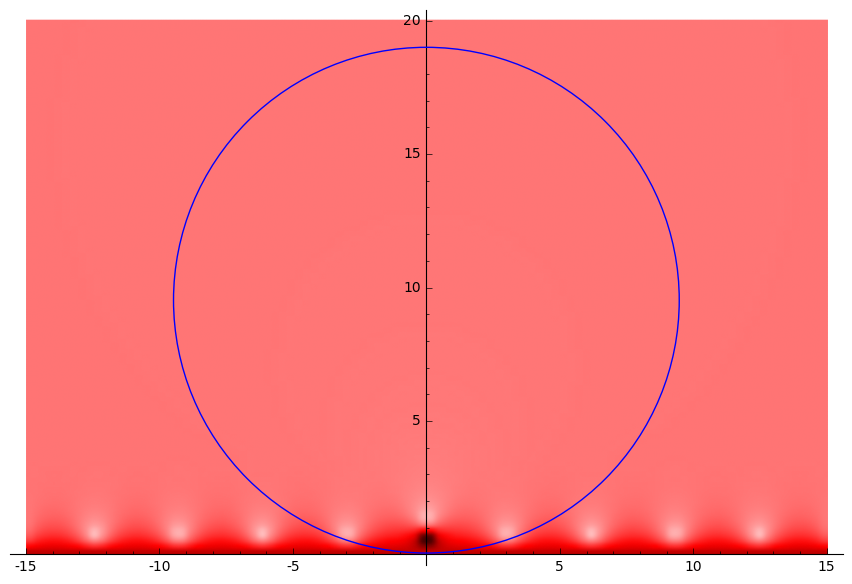
\includegraphics[width=\textwidth,height=\textheight,keepaspectratio]{pic/contour_white.png}
{\caption{$\abs{\det S(k)}^{-1}$. Резонатор типа «пучок» ($W = 2$, $a = 1$, $b = -2$); $r = 0.9$}}
% (complex_plot(abs(S), (-15, 15), (0, 20)) + circle((0, 7), 6.5)).show(figsize=[12, 6], aspect_ratio='equal')
\end{figure}
\end{frame}
% SAY Проблема в том, что контур интегрирования может пересекать особенности


\begin{frame}{Резонатор типа «кольцо»}

\begin{figure}
\begin{tikzpicture}[scale=0.8]
\newcommand{\Wglen}{6.0}; % waveguide length
\newcommand{\Warrlen}{2.0}; % wave arrow length
\newcommand{\Reslen}{0.0}; % resonator length

\coordinate (LLL) at (-\Wglen - 1, 0);
\coordinate (RRR) at ( \Wglen + 1, 0);
\coordinate (LL)  at (-\Wglen, 0);
\coordinate (RR)  at ( \Wglen, 0);
\coordinate (L)   at (-\Reslen, 0);
\coordinate (R)   at ( \Reslen, 0);
%

\coordinate (U) at (0, 3); % upper point of resonator

% waveguide
\draw[ultra thick, dotted] (LLL) -- (LL);
\draw[ultra thick] (LL)--(L);
\draw[ultra thick] (R)--(RR);
\draw[ultra thick, dotted] (RR) -- (RRR);
%

\draw[<-, thick] (-\Wglen, 1.5) -- (-\Wglen + \Warrlen, 1.5) node [midway, above] {\large $R e^{-\iu k x}$};
\draw[->, thick] (-\Wglen, 0.8) -- (-\Wglen + \Warrlen, 0.8) node [midway, above] {\large $e^{\iu k x}$};
\draw[->, thick] (\Wglen - \Warrlen, 0.5) -- (\Wglen, 0.5)   node [midway, above] {\large $T e^{\iu k x}$};

\draw (LL) node [below] {\large $\Omega_L$};
\draw (RR) node [below] {\large $\Omega_R$};

\draw[ultra thick] (0, 2) node [above] {\Large $\Omega$};

\draw[ultra thick] node [below] {\large $V$} (0, 2) circle[radius=2];
\end{tikzpicture}
\end{figure}

\[
\det S = 
\frac
{\cos\left(k\right) + {\left(\frac{a}{2 k} + i\right)} \sin\left(k\right) - 1}
{\cos\left(k\right) + {\left(\frac{a}{2 k} - i\right)} \sin\left(k\right) - 1}
\]

\end{frame}

\begin{frame}{Резонатор типа «кольцо»}
\begin{itemize}
\item $a = 0$: полноты нет, $\det S$ слишком быстро уходит в 0 на бесконечности ($\log \det S(k) = \mcO(\Im k))$)
\item $a \ne 0$: полнота присутствует, $\det S$ все еще уходит в 0, но не так быстро: ($\log \det S(k) = \mcO(\log \Im k))$)
\end{itemize}
\end{frame}

% \begin{frame}[plain]
% \begin{figure}
% 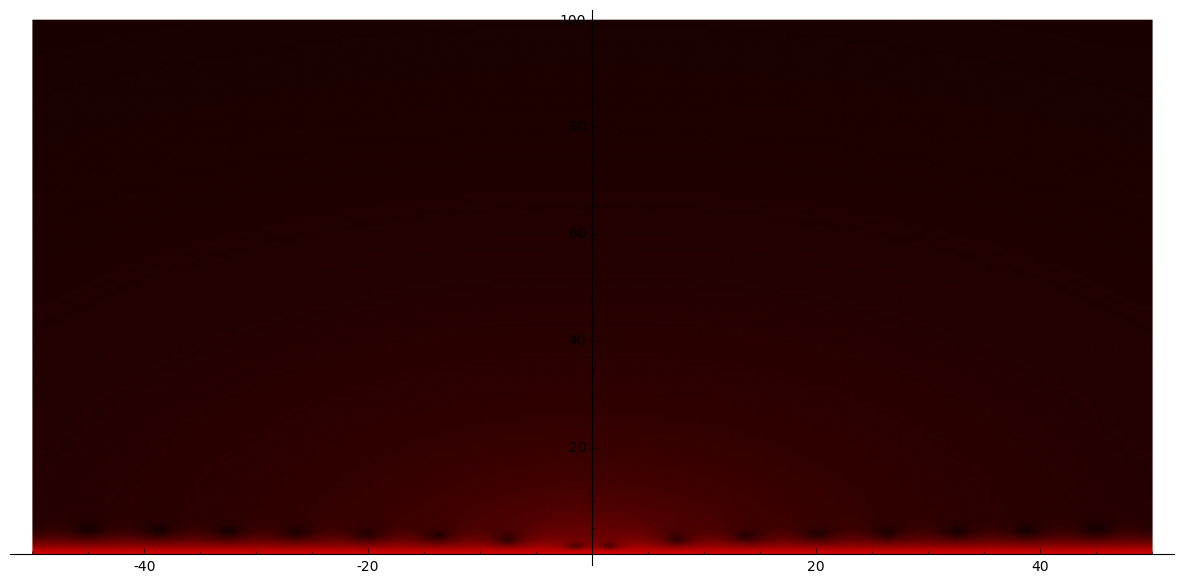
\includegraphics[width=\textwidth,height=\textheight,keepaspectratio]{pic/detSa1.png}
% \caption{$\abs{\det S(k)}$, $a = 1$}
% \end{figure}
% \end{frame}


% TODO meh. Просто упомянуть?
% \begin{frame}{Резонатор типа «кольцо с петлей»}

% \end{frame}

\begin{frame}{Схема доказательства полноты}

\[
\lim\limits_{r \to 1} \int\limits_{0}^{2 \pi} \ln \abs{\det S(k)} \frac{R}{(R(r) \eexp{\iu t} + \iu C(r) + i)^2} dt = 0
\]

Используем неравенство Коши-Буняковского: $\big| \langle f,g \rangle \big| \leq \left\|f\right\| \left\|g\right\|$

\begin{align*}
f(t)   &= \ln \abs{\det S(k)} \frac{\sqrt{R}}{R \eexp{\iu t} + \iu C + i} \\
g^*(t) &= \frac{\sqrt{R}}{R \eexp{\iu t} + \iu C + i}
\end{align*}

\begin{align*}
\norm{g} &\le \pi \\
\lim_{R \to \infty} \norm{f} &= 0
\end{align*}
\end{frame}



\begin{frame}{Резонатор типа «пучок» из $W$ одинаковых ребер}

\begin{figure}
\begin{tikzpicture}[scale=0.8]
\newcommand{\Wglen}{6.0}; % waveguide length
\newcommand{\Warrlen}{2.0}; % wave arrow length
\newcommand{\Reslen}{4.0}; % resonator length

\coordinate (LLL) at (-\Wglen - 1, 0);
\coordinate (RRR) at ( \Wglen + 1, 0);
\coordinate (LL)  at (-\Wglen, 0);
\coordinate (RR)  at ( \Wglen, 0);
\coordinate (L)   at (-\Reslen, 0);
\coordinate (R)   at ( \Reslen, 0);
%

\coordinate (U) at (0, 3); % upper point of resonator

% waveguide
\draw[ultra thick, dotted] (LLL) -- (LL);
\draw[ultra thick] (LL)--(L);
\draw[ultra thick] (R)--(RR);
\draw[ultra thick, dotted] (RR) -- (RRR);
%

\draw[<-, thick] (-\Wglen, 1.5) -- (-\Wglen + \Warrlen, 1.5) node [midway, above] {\large $R e^{-\iu k x}$};
\draw[->, thick] (-\Wglen, 0.8) -- (-\Wglen + \Warrlen, 0.8) node [midway, above] {\large $e^{\iu k x}$};
\draw[->, thick] (\Wglen - \Warrlen, 0.5) -- (\Wglen, 0.5)   node [midway, above] {\large $T e^{\iu k x}$};

\draw (LL) node [below] {\large $\Omega_L$};
\draw (RR) node [below] {\large $\Omega_R$};

\draw[ultra thick] (0, 2) node [above] {\Large $\Omega$};

% \draw[ultra thick] node [below] {$V$} (0, 2) circle[radius=2] 
\draw[thick] (4,0)  arc[x radius = 4cm, y radius = 2cm, start angle= 0, end angle=180];
\draw[thick] (4,0)  arc[x radius = 4cm, y radius = 1cm, start angle= 0, end angle=180];
\draw[thick] (4,0)  arc[x radius = 4cm, y radius = 0.5cm, start angle= 0, end angle=180];
\draw[thick] (-4,0)  arc[x radius = 4cm, y radius = 2cm, start angle= 180, end angle=360];
\draw[thick] (-4,0)  arc[x radius = 4cm, y radius = 1cm, start angle= 180, end angle=360];
\draw[thick] (-4,0)  arc[x radius = 4cm, y radius = 0.5cm, start angle= 180, end angle=360];

\draw (-\Reslen - 0.3, 0) node [below] {\large $V_a$};
\draw ( \Reslen + 0.3, 0) node [below] {\large $V_b$};
\draw (0, 0) node {\large $\dots$};
\end{tikzpicture}
\end{figure}

\end{frame}


\begin{frame}{Резонатор типа «пучок» из $W$ одинаковых ребер}

{
\scriptsize
\[
\det S(k) = \frac{W {\left(a + b\right)} k \cos\left(k\right) + 2 i \, W k^{2} \cos\left(k\right) + {\left(i \, a + i \, b\right)} k \sin\left(k\right) - {\left({\left(W^{2} + 1\right)} k^{2} - a b\right)} \sin\left(k\right)}{W {\left(a + b\right)} k \cos\left(k\right) - 2 i \, W k^{2} \cos\left(k\right) - {\left(i \, a + i \, b\right)} k \sin\left(k\right) - {\left({\left(W^{2} + 1\right)} k^{2} - a b\right)} \sin\left(k\right)}
\]
}

\[
f(t) =  \mcO\left( \frac{\ln^3 R}{\sqrt{R}} \right)
\]
\end{frame}

% Since $S$-matrix is naturally defined on the complex plane, it is easier work in the upper complex plane. To do that, we apply the Cayley transorm $W(z) = \frac{z - \iu}{z + \iu}$, which maps upper complex plane to the unit disk, and its inverse $w(\zeta) = \iu \frac{1 + \zeta}{1 - \zeta}$, which yields:

% \begin{equation}\label{crit}
% \lim\limits_{r \to 1} \int\limits_{C_r} \ln \abs{\det S(k)} \frac{2 \iu}{(k + i)^2} dk = 0
% \end{equation}

% , where $C_r$ is the image of the curve $\abs{\zeta} = r$ under the inverse Cayley transform. Since Cayley transform is a Mobius transformation and preserves circles, $C_r$ will actually be a circle with radius $R(r) = \Im \frac{w(r) - w(-r)}{2}$ and center $C(r) = \Im \frac{w(r) + w(-r)}{2}$.

% Fox the computational convenience, it $C_r$ is parameterized via $k = R(r) \eexp{\iu t} + \iu C(r)$, which yields us the final form of the criterion, which we will use further:

% \begin{equation}\label{critp}
% \lim\limits_{r \to 1} \int\limits_{0}^{2 \pi} \ln \abs{\det S(R(r) \eexp{\iu t} + \iu C(r))} \frac{2 \iu}{(R(r) \eexp{\iu t} + \iu C(r) + i)^2} R \iu dt = 0
% \end{equation}




\begin{frame}{Доказательство для произвольного графа}
Хотелось бы использовать индукцию по количеству ребер.

Но при «стягивании» ребер можно потерять полноту. % \todo{$S$-матрица в пределе?}
% интересный результат: непрерывное изменение параметров приводит к внезапному разрыву 
% возможно, необходим другой подход или более сложный инвариант индукции
\end{frame}


\begin{frame}{Резонатор из двух проводов разной длины}

\begin{figure}
\begin{tikzpicture}[scale=0.8]
\newcommand{\Wglen}{6.0}; % waveguide length
\newcommand{\Warrlen}{2.0}; % wave arrow length
\newcommand{\Reslen}{4.0}; % resonator length

\coordinate (LLL) at (-\Wglen - 1, 0);
\coordinate (RRR) at ( \Wglen + 1, 0);
\coordinate (LL)  at (-\Wglen, 0);
\coordinate (RR)  at ( \Wglen, 0);
\coordinate (L)   at (-\Reslen, 0);
\coordinate (R)   at ( \Reslen, 0);
%

\coordinate (U) at (0, 3); % upper point of resonator

% waveguide
\draw[ultra thick, dotted] (LLL) -- (LL);
\draw[ultra thick] (LL)--(L);
\draw[ultra thick] (R)--(RR);
\draw[ultra thick, dotted] (RR) -- (RRR);
%

\draw[<-, thick] (-\Wglen, 1.5) -- (-\Wglen + \Warrlen, 1.5) node [midway, above] {\large $R e^{-\iu k x}$};
\draw[->, thick] (-\Wglen, 0.8) -- (-\Wglen + \Warrlen, 0.8) node [midway, above] {\large $e^{\iu k x}$};
\draw[->, thick] (\Wglen - \Warrlen, 0.5) -- (\Wglen, 0.5)   node [midway, above] {\large $T e^{\iu k x}$};

\draw (LL) node [below] {\large $\Omega_L$};
\draw (RR) node [below] {\large $\Omega_R$};

\draw[ultra thick] (0, 2) node [above] {\Large $\Omega$};

% \draw[ultra thick] node [below] {$V$} (0, 2) circle[radius=2] 
\draw[thick] (4,0)  arc[x radius = 4cm, y radius = 2cm, start angle= 0, end angle=180];
\draw[thick] (L)--(R);
% \draw[thick] (4,0)  arc[x radius = 4cm, y radius = 1cm, start angle= 0, end angle=180];
% \draw[thick] (4,0)  arc[x radius = 4cm, y radius = 0.5cm, start angle= 0, end angle=180];
% \draw[thick] (-4,0)  arc[x radius = 4cm, y radius = 2cm, start angle= 180, end angle=360];
% \draw[thick] (-4,0)  arc[x radius = 4cm, y radius = 1cm, start angle= 180, end angle=360];
% \draw[thick] (-4,0)  arc[x radius = 4cm, y radius = 0.5cm, start angle= 180, end angle=360];

\draw (-\Reslen - 0.3, 0) node [below] {\large $V_a$};
\draw ( \Reslen + 0.3, 0) node [below] {\large $V_b$};
\draw (0, 0) node [below] {\large $L$};
\end{tikzpicture}
\end{figure}


\[
\det S(k) = 
\frac{
(2 \cos k  + 2 \iu \sin k) \cos(L k) + (2 \iu \cos k  - 3 \sin k) \sin(L k) - 2
}
{
(2 \cos k  - 2 \iu \sin k) \cos(L k) + (-2 \iu \cos k  - 3 \sin k) \sin(L k) - 2
}
\]

Полнота есть при любом $L \ne 0$!
% SAY L = 0 — то же самое, что случай с кольцом

\end{frame}


\begin{frame}{Заключение}
\begin{itemize}
\item Построена $S$-матрица в аналитическом виде для различных квантовых графов
\item Исследована полнота резонансных функций и показано качественно различное поведение при изменении параметров и граничных условий систем
\end{itemize}
\end{frame}


\begin{frame}{Публикации}
\begin{itemize}
\item \fullcite{sbornik}
\item \fullcite{diffdays}
% SAY about almost ready paper?
\end{itemize}
\end{frame}

\end{document}